%Author Cesar
%Desc : For my presentations


\documentclass{beamer}\usetheme{Madrid} %

\setbeamercovered{invisible} % To remove the navigation symbols from
% the bottom of slides%
%\setbeamertemplate{navigation symbols}{}  %Disable the navigation
%

\usepackage{upquote} %proper quotation inside the verbatim

% sudo apt-get install texlive-full or texlive-science (the latter is minimal)
\usepackage{algorithmic}
\usepackage[spanish]{babel} 
\usepackage{algorithm2e}
\usepackage{color}
\usepackage{fancyvrb}

\usepackage{boxedminipage} %modified Madrid footer
\usepackage{graphicx}
\usepackage{caption}
%\usepackage{bm}         % For typesetting bold math (not \mathbold)
%\logo{\includegraphics[height=0.6cm]{yourlogo.eps}}
%
\usepackage{amsmath}

\title[ACR]{Adaptive Code Refinement}
\author{C\'esar Sabater} \institute[UNR] {
%University of Strasbourg \\

\medskip
%{\emph{aravind.sukumaran-rajam@inria.fr}}\\
%\vspace{10px}
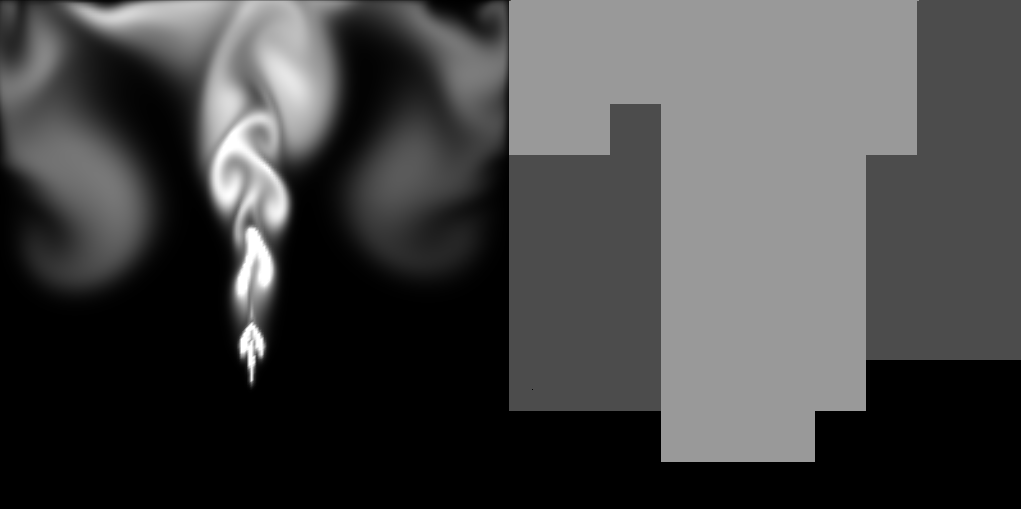
\includegraphics[scale=0.1]{img/logo.png} }

\subject{ Presentaci\'on Tesina 2017 } % \tiny{ }

\date{ \today} % \today will show
%current date.

\setbeamertemplate{navigation symbols}{}%remove navigation symbols 

%custom beaver footnote do what ever u want
\setbeamertemplate{footline} {%
\leavevmode
%
\hbox{%
\begin{beamercolorbox}[wd=.323\paperwidth,ht=2.25ex,dp=1ex,center]
    {author in head/foot}%
    \usebeamerfont{author in head/foot} Universidad Nacional de Rosario
\end{beamercolorbox}
%
\begin{beamercolorbox}[wd=.333\paperwidth,ht=2.25ex,dp=1ex,center]
    {title in head/foot}%
    \usebeamerfont{title in head/foot}\insertshorttitle
\end{beamercolorbox}
%
\begin{beamercolorbox}[wd=.3333\paperwidth,ht=2.25ex,dp=1ex,right]
    {date in head/foot}%
    \usebeamerfont{date in head/foot}\insertshortdate{}\hspace*{2em}
    \insertframenumber{} / \inserttotalframenumber\hspace*{1ex}
\end{beamercolorbox}
}%
\vskip0pt%
}

%\logo{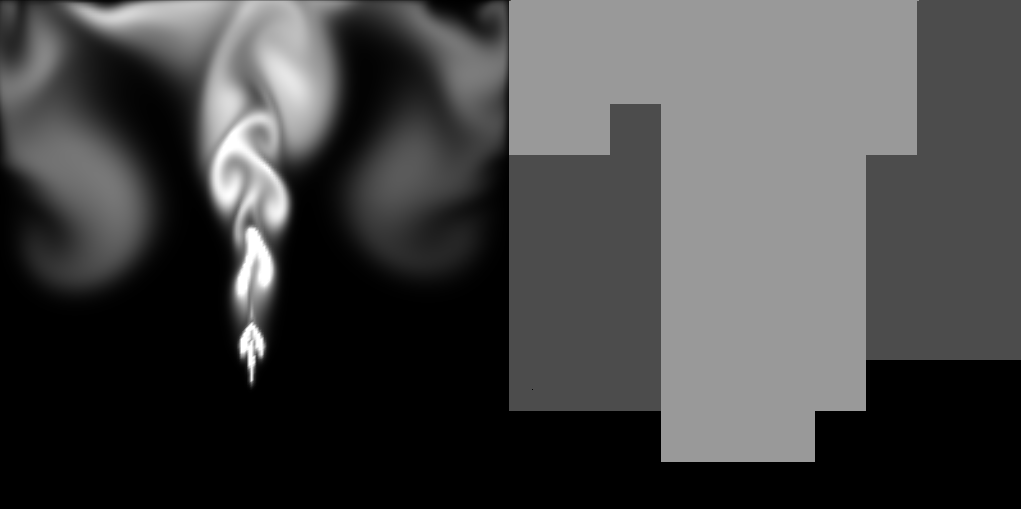
\includegraphics[scale=.04]{img/logo.png}}

\newcommand\codeHighlight[1]{\textcolor[rgb]{1,0,0}{\textbf{#1}}}

\newenvironment{rcases} {\left.
\begin{aligned}
    } {%
\end{aligned}
\right\rbrace}

\begin{document}
%
{ \setbeamertemplate{logo}{}
\begin{frame}
    \titlepage
    \vspace*{-25px}
    \begin{center}
        \large{ Presentaci\'on de Tesina }
    \end{center}

\end{frame}
}

%%%%%%%%%%%%%%%%%%%%%%%%%%%%%%%%%%%%%%%%%%%%%%%%%%%%%%%%%%%%%%%%%%%%%%%%%%%%%%%%
\begin{frame}
    \frametitle{Simulation}
    %more concrete simualtions, but a more abstract kind of problem
    \begin{itemize}
        \item
			A simulation is a program that immitates the behavior of a system over time
		\item
			It implements the abstract model describing the system
		\item
			\textbf{Usssually, it requires a big ammount of computing power }
    \end{itemize}
    	\begin{figure} 
	 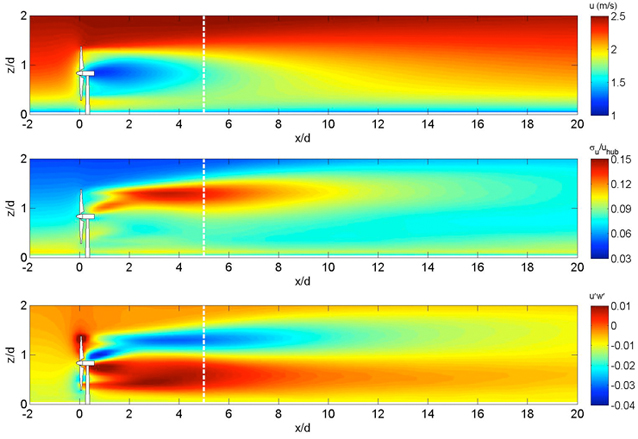
\includegraphics[scale=0.18]{img/wind_sim.jpg}
    \end{figure}
\end{frame}
%%%%%%%%%%%%%%%%%%%%%%%%%%%%%%%%%%%%%%%%%%%%%%%%%%%%%%%%%%%%%%%%%%%%%%%%%%%%%%%%
\begin{frame}
    \frametitle{Optimizing Simulation}
    \begin{itemize}
				\item 
					Preserving accuracy:
					\begin{itemize}
						\item
							paralellization
						\item
							data locality
						\item
							loop reordering
						\item
							vectorization
						\item
							\textcolor{blue}{well addressed by automatic approaches}
						\end{itemize}
				\item
					Not preserving accuracy
						\begin{itemize}
						\item 
							less precise models
						\item
							less accurate computations
						\item
							adaptive mesh refinement
						\item
							\textcolor{red}{not well addressed by automatic approaches}
						\end{itemize}				
    \end{itemize}
    \textbf{Our goal:} to design a compiler approach to optimize simulation codes
    \begin{itemize}
		\item
			by tuning accuracy
		\item
			through adaptive techniques
		\end{itemize}
\end{frame}
%%%%%%%%%%%%%%%%%%%%%%%%%%%%%%%%%%%%%%%%%%%%%%%%%%%%%%%%%%%%%%%%%%%%%%%%%%%%%%%%
\begin{frame}
    \frametitle{Outline} 
    \begin{itemize}
		\item
			Aimed Simulation: Eulerian Fluid Simulation
        \item
            Adaptive Techniques
        \item
            Static Tool: Spot
        \item
            Dynamic Tool: Adaptive Code Refinement
        \item
            Experiments
    \end{itemize}
\end{frame}
%%%%%%%%%%%%%%%%%%%%%%%%%%%%%%%%%%%%%%%%%%%%%%%%%%%%%%%%%%%%%%%%%%%%%%%%%%%%%%%%
\begin{frame}
\frametitle { Eulerian Fluid Simulation }
\begin{columns} 
\column[t]{0.50\textwidth}
\begin{itemize}
	\item
		Simulates the behavior of a fluid over time
	\item
		A rectangle is divided into cells, and every cell represent a 
		particle
	\item
		At every time iteration, every cell actualizes its density value
		and its velocity vector
\end{itemize}
\column[t]{0.40\textwidth}
%~ \begin{columns} 
%~ \column[t]{0.45\textwidth}
\begin{figure}
        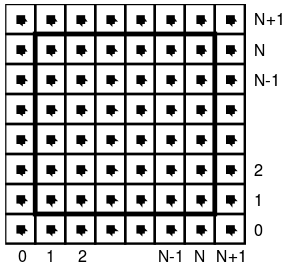
\includegraphics[scale=0.18]{img/eul1.png}
        %         \caption { AMR for Shock Hydrodynamics  }
    \end{figure}
%~ \column[t]{0.45\textwidth}
\begin{figure}
        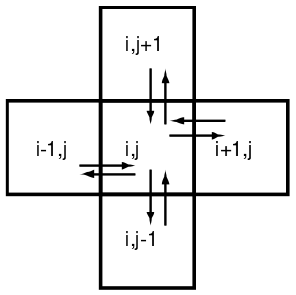
\includegraphics[scale=0.18]{img/eul3.png}
%         \caption { AMR for Shock Hydrodynamics  }
\end{figure}
%~ \end{columns}
\end{columns}
\begin{figure}
        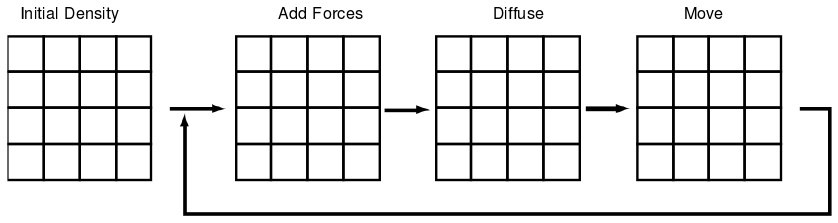
\includegraphics[scale=0.32]{img/eul2.png}
%         \caption { AMR for Shock Hydrodynamics  }
\end{figure}
\end{frame}
%%%%%%%%%%%%%%%%%%%%%%%%%%%%%%%%%%%%%%%%%%%%%%%%%%%%%%%%%%%%%%%%%%%%%%%%%%%%%%%%
\begin{frame}
    \frametitle{Adaptive Techniques} An adaptive technique only performs computations only 
		where it is needed in the iteration space
			\begin{itemize}
						\item
							It changes the way it operates depending on the input
						\item
							It doesn't spends unnecesary computations
						\item
							It develops different regions of interest on computation
						\item
							It changes its behavior over time to fit the new states
							of the execution
    \end{itemize}
\end{frame}
%%%%%%%%%%%%%%%%%%%%%%%%%%%%%%%%%%%%%%%%%%%%%%%%%%%%%%%%%%%%%%%%%%%%%%%%%%%%%%%%
\begin{frame}
  \frametitle {Example: Adaptive Mesh Refinement} AMR is a Numerical Analysis technique for changing the accuracy
		of a solution in certain regions, while the solution is being calculated
   \begin{columns}
	 \column[t]{0.45\textwidth}
    \begin{itemize}
		\item 
			It computes hierarchical grid wich specifies the complexity
			of the computation
		\item
			It refines the precision of the calculation in intresting
			regions
		\item
			It performs basic calculations in regions where almost nothing
			or nothing hapens
    \end{itemize}
    \column[t]{0.45\textwidth}
    \begin{figure}
        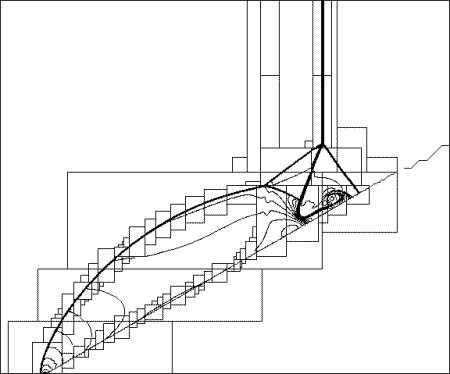
\includegraphics[scale=0.32]{img/Amrgridimg2.jpg}
        %         \caption { AMR for Shock Hydrodynamics  }
    \end{figure}
		\end{columns}
\end{frame}
%%%%%%%%%%%%%%%%%%%%%%%%%%%%%%%%%%%%%%%%%%%%%%%%%%%%%%%%%%%%%%%%%%%%%%%%%%%%%%%%
\begin{frame}
    \frametitle { First Approach: Static Accuracy Tuning }
    \begin{columns}
    \column[t]{0.45\textwidth}
    \begin{itemize}
		\item
			we want to apply a filter the image
		\item
			the important region of the image is the flower
		\item
			the rest of the image can be processed by some simple 
			calculations
	\end{itemize}
    \column[t]{0.45\textwidth}
		\begin{figure}
			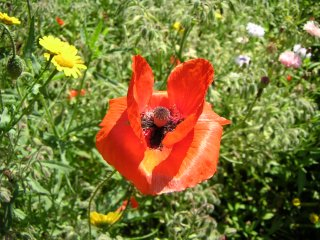
\includegraphics[scale=0.32]{img/rose.jpg}
			%         \caption { AMR for Shock Hydrodynamics  }
		\end{figure}
    \end{columns}
\end{frame}
%%%%%%%%%%%%%%%%%%%%%%%%%%%%%%%%%%%%%%%%%%%%%%%%%%%%%%%%%%%%%%%%%%%%%%%%%%%%%%%%
\begin{frame}
    \frametitle {SPOT} Simple Polyhedral loop Transformer
    \begin{itemize}
	\item 
		source-to-source compilation tool for transforming loops
	\item
		allows us to input to a program information of different regions
		of a computation space
	\item
		manipulates the iteration space of a loop to change/eliminate 
		computations in regions specified in pragmas
    \end{itemize}
\end{frame}
%%%%%%%%%%%%%%%%%%%%%%%%%%%%%%%%%%%%%%%%%%%%%%%%%%%%%%%%%%%%%%%%%%%%%%%%%%%%%%%%
\begin{frame}[fragile]
\frametitle { SPOT } Example: Image Processing
\begin{verbatim}
#pragma spot 1
   "[H, W]->{[x,y]: x > 3*H/4 or y > 3*W/4 or x < H/4 or y > W/4}" 
   "simpleFilter(x, y, IMG);"
for (x = 0; x < H; x++) 
   for (y = 0; y < W; y++)
      complexFilter(x, y, IMG);
\end{verbatim}
\begin{columns}
\column[t]{0.45\textwidth}
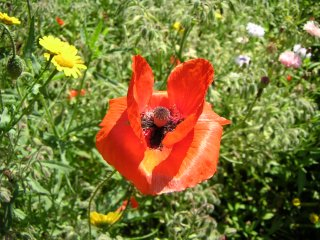
\includegraphics[scale=0.32]{img/rose.jpg}
			%         \caption { AMR for Shock Hydrodynamics  }
\column[t]{0.45\textwidth}
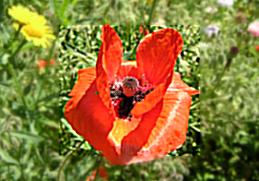
\includegraphics[scale=0.43]{img/flower_proc.png}
			%         \caption { AMR for Shock Hydrodynamics  }
\end{columns}
\end{frame}
%%%%%%%%%%%%%%%%%%%%%%%%%%%%%%%%%%%%%%%%%%%%%%%%%%%%%%%%%%%%%%%%%%%%%%%%%%%%%%%%
\begin{frame}
    \frametitle { SPOT } Simple Polyhedral loop Transformer
    \begin{itemize}
		\item 
			uses ISL to specify input regions in pragmas as integer sets
		\item
			relies on polyhedral tools to analyze and process the sets
		\item 
			it generates new code that performs the computations 
			specified in the different regions
    \end{itemize}
\end{frame}
%%%%%%%%%%%%%%%%%%%%%%%%%%%%%%%%%%%%%%%%%%%%%%%%%%%%%%%%%%%%%%%%%%%%%%%%%%%%%%%%
\begin{frame}[fragile]
\frametitle { SPOT } Simple Polyhedral loop Transformer
\begin{verbatim}
#pragma spot 1 
    "[N1, N2]->{[i,j]: i < N1/2 and j < N2/2}" 
    "COMPUTATION1"
#pragma spot 2 
	"[N1, N2]->{[i,j]: i > N1/2 and j > N2/2}" 
	"COMPUTATION2"
for (i = 0; i < N1; i++) 
   for (j = 0; j < N2; j++)
      ORIGINAL COMPUTATIONS;
\end{verbatim}
\end{frame}
%%%%%%%%%%%%%%%%%%%%%%%%%%%%%%%%%%%%%%%%%%%%%%%%%%%%%%%%%%%%%%%%%%%%%%%%%%%%%%%%
\begin{frame}
\begin{columns}
\column[t]{0.45\textwidth}
\begin{figure}
        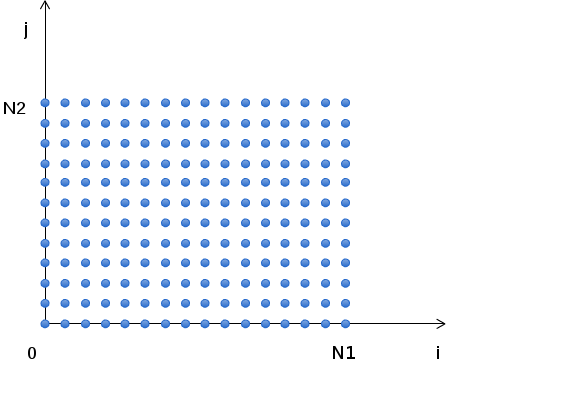
\includegraphics[scale=0.35]{img/itspace-white.png}
 %         \caption { AMR for Shock Hydrodynamics  }
\end{figure}
\column[t]{0.45\textwidth}
\begin{figure}
    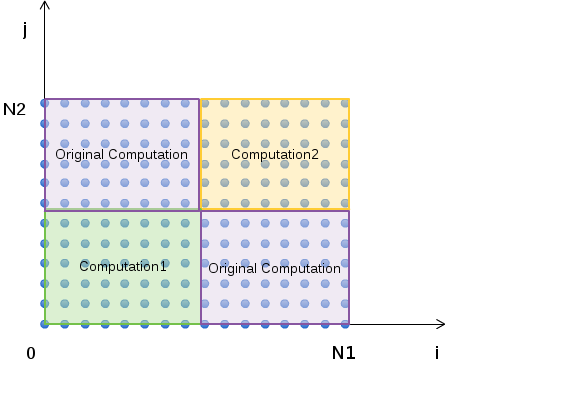
\includegraphics[scale=0.35]{img/itspace_trans-white.png}
   %         \caption { AMR for Shock Hydrodynamics  }
\end{figure}
\end{columns}
\end{frame}
%%%%%%%%%%%%%%%%%%%%%%%%%%%%%%%%%%%%%%%%%%%%%%%%%%%%%%%%%%%%%%%%%%%%%%%%%%%%%%%%
\begin{frame}
\frametitle { Adaptive Code Refinement } 
\begin{itemize}
		\item 
			provide adaptive capabilities to simulation codes
		\item
			uses domain-specific knowledge
			\begin{itemize}
			\item 
				save unnecesary computations
			\item	
				achieves "good enough results"
			\end{itemize}
		\item 
			regenerates the code in execution time
		\item 
			uses SPOT to process iteration portions and to generate code
\end{itemize}
\end{frame}
%%%%%%%%%%%%%%%%%%%%%%%%%%%%%%%%%%%%%%%%%%%%%%%%%%%%%%%%%%%%%%%%%%%%%%%%%%%%%%%
\begin{frame}
\frametitle { Adaptive Code Refinement: How it works } 
\begin{itemize}
		\item 
			uses a grid to gather useful information about the simulation 
			state
		\begin{itemize}
			\item 
				complexity of computation needed in every region
			\item 
				grid processing is lightweight
			\end{itemize}
		\item 
			generates an optimized version of code according to the grid
		\item 
			when the grid changes, the code is regenerated
\end{itemize}
\end{frame}
%%%%%%%%%%%%%%%%%%%%%%%%%%%%%%%%%%%%%%%%%%%%%%%%%%%%%%%%%%%%%%%%%%%%%%%%%%%%%%%%
\begin{frame}[fragile]
\frametitle { ACR }  
\begin{verbatim}
for (time = 0; time < T; time++) 
 #pragma ACR	gridsize=6 
 {S1 -> Complex(i,j,t), S2 -> Simple(i,j,t), 
   S3 -> AlmostNothing(i,j,t)}
 for (i = 0; i < N; i++) 
   for (j = 0; j < N; j++) { 
     Original(i,j,t);
   }
\end{verbatim}
\begin{figure}
        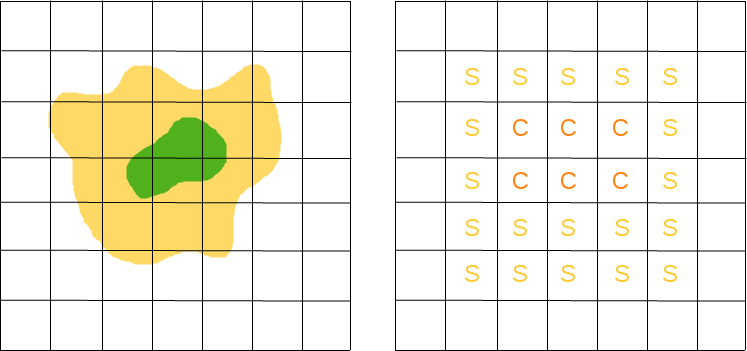
\includegraphics[scale=0.25]{img/grid-w.png}
 %         \caption { AMR for Shock Hydrodynamics  }
\end{figure}
\end{frame}
%%%%%%%%%%%%%%%%%%%%%%%%%%%%%%%%%%%%%%%%%%%%%%%%%%%%%%%%%%%%%%%%%%%%%%%%%%%%%%%%
\begin{frame}
\frametitle { ACR } Threads
\begin{itemize}
	\item
		Simulation and Code generation are done in two parallel threads
	\item
		One thread executes the simulation code available and refreshes 
		the grid
	\item
		The other thread recompiles the simulation code when the grid 
		changes
\end{itemize}
	\begin{figure}
        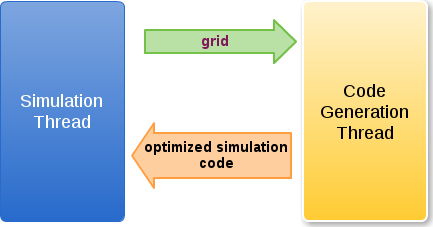
\includegraphics[scale=0.50]{img/threads-w.png}
%         \caption { AMR for Shock Hydrodynamics  }
\end{figure}
\end{frame}
%%%%%%%%%%%%%%%%%%%%%%%%%%%%%%%%%%%%%%%%%%%%%%%%%%%%%%%%%%%%%%%%%%%%%%%%%%%%%%%%
\begin{frame}
\frametitle { ACR } Ensuring "Safety" 
\begin{itemize}
	\item
		there is a gap between grid change and new code available
	\item
		if the available optimized code doesn't fit the current grid
		the simulation thread executes the original code
	\item
		to avoid to many switches to the original code, the surroundings
		of intrest regions are also covered by the grid
\end{itemize}
\end{frame}
%%%%%%%%%%%%%%%%%%%%%%%%%%%%%%%%%%%%%%%%%%%%%%%%%%%%%%%%%%%%%%%%%%%%%%%%%%%%%%%%
\begin{frame}
\frametitle { Experiments } 2D Eulerian Fluid Simulation
\begin{itemize}
	\item
		Simulates the behavior of a fluid over time
	\item
		A rectangle is divided into cells, and every cell represent a 
		particle
	\item
		At every time iteration, every cell actualizes its density value
		and its velocity vector
\end{itemize}
\end{frame}
%%%%%%%%%%%%%%%%%%%%%%%%%%%%%%%%%%%%%%%%%%%%%%%%%%%%%%%%%%%%%%%%%%%%%%%%%%%%%%%%
\begin{frame}
\frametitle { Experiments } Applying ACR
\begin{itemize}
	\item
		The complexity of the computation in a region depends on
		the density of the fluid
	\item
		As the simulation evolves, the grid will adapt to fit complex
		calculations where the fluid is
	\item
		More simpler calculations will be done where there is a little
		amount of fluid, and almost any where there is not fluid
\end{itemize}
\end{frame}
%%%%%%%%%%%%%%%%%%%%%%%%%%%%%%%%%%%%%%%%%%%%%%%%%%%%%%%%%%%%%%%%%%%%%%%%%%%%%%%%
\begin{frame}
\frametitle { Experiments } 
\begin{columns}
\column[t]{0.45\textwidth}
\begin{figure}
        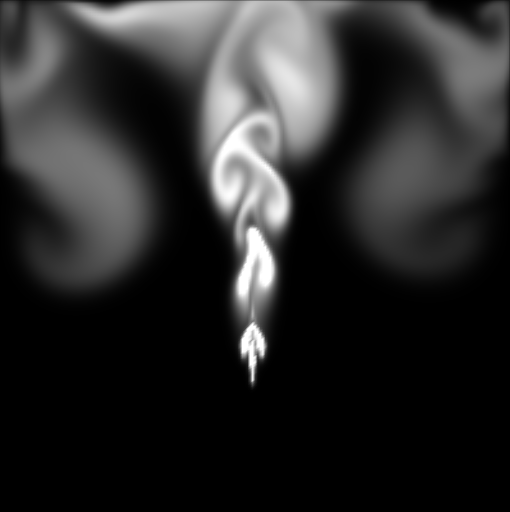
\includegraphics[scale=0.28]{img/simulation.png}
 %         \caption { AMR for Shock Hydrodynamics  }
\end{figure}
\column[t]{0.45\textwidth}
\begin{figure}
    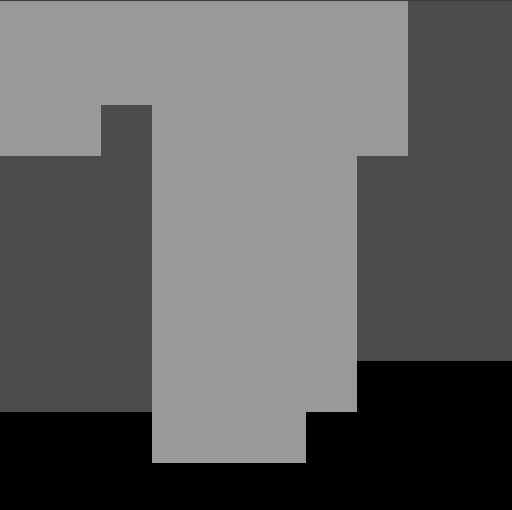
\includegraphics[scale=0.28]{img/sim_grid.png}
   %         \caption { AMR for Shock Hydrodynamics  }
\end{figure}
\end{columns}
\end{frame}
%%%%%%%%%%%%%%%%%%%%%%%%%%%%%%%%%%%%%%%%%%%%%%%%%%%%%%%%%%%%%%%%%%%%%%%%%%%%%%%%
\begin{frame}
\frametitle { Results: Saved Computations }
\begin{figure}
    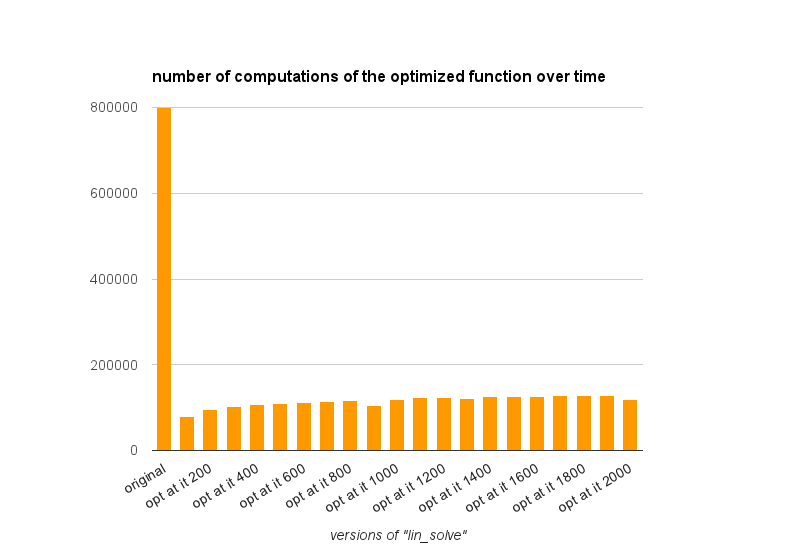
\includegraphics[scale=0.40]{img/computations.png}
\end{figure}
\end{frame}
%%%%%%%%%%%%%%%%%%%%%%%%%%%%%%%%%%%%%%%%%%%%%%%%%%%%%%%%%%%%%%%%%%%%%%%%%%%%%%%%
\begin{frame}
\frametitle { Results: Performance over time }
\begin{figure}
    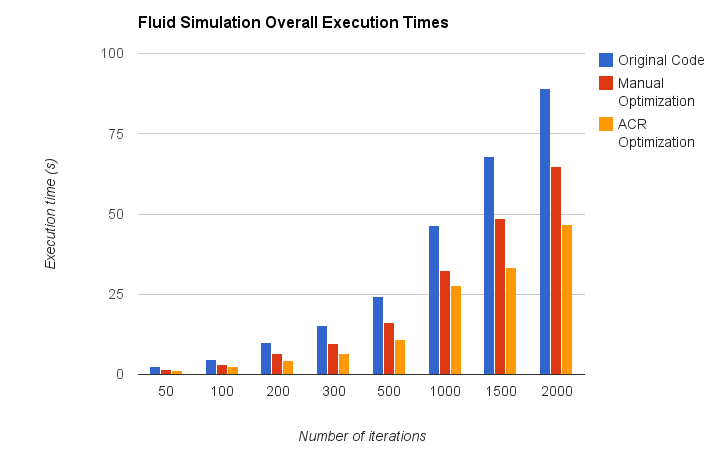
\includegraphics[scale=0.60]{img/times.png}
\end{figure}
\end{frame}
%%%%%%%%%%%%%%%%%%%%%%%%%%%%%%%%%%%%%%%%%%%%%%%%%%%%%%%%%%%%%%%%%%%%%%%%%%%%%%%%
\begin{frame}
\frametitle { Results: Accuracy }
\begin{figure}
    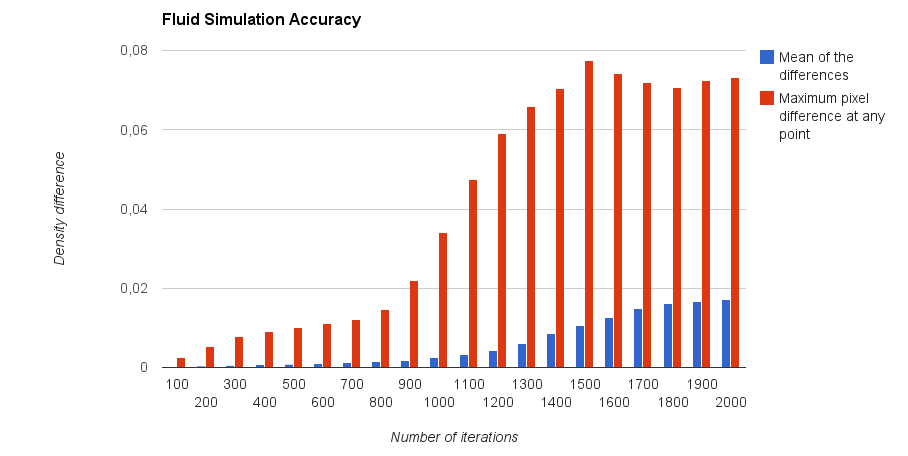
\includegraphics[scale=0.40]{img/accuracy.png}
\end{figure}
\end{frame}
%%%%%%%%%%%%%%%%%%%%%%%%%%%%%%%%%%%%%%%%%%%%%
\begin{frame}
    \centerline{Questions?}
\end{frame}
% End of slides
\end{document}



